	\chapter{Statistics}
	\formattedepigraph{All models are wrong, but some models are useful.}{George Box}

The five characteristic numbers:
	\begin{plainlist}
		\item \xsmallest{}
		\item \quartileone{}
		\item \quartiletwo{}
		\item \quartilethree{}
		\item \xlargest{}
	\end{plainlist}

Box plot, maximum 1.5 times interquartile range.  The rest are outliers and plot them accordingly.



median formula?
	\begin{eqnarray}
		\variance 					& = & \frac{1}{N-1}\sum^N_{i=1}\left(x_i - \samplemean\right)^2 \\
		\samplestandarddeviation	& = & \sqrt{\variance}
	\end{eqnarray}
Note that this version assumes equal probability of all data.



coefficient of variation

	\begin{figure}[tbp]
		\centering
		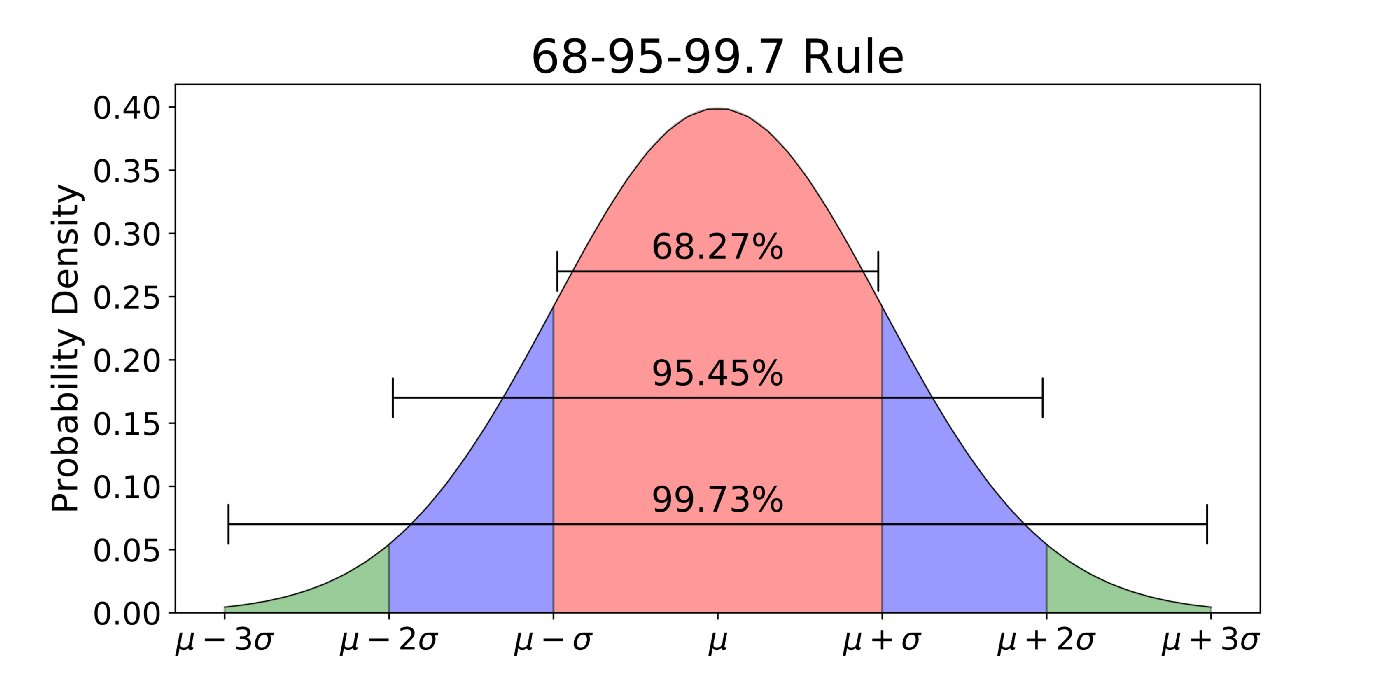
\includegraphics[height=2.5in]{normaldistrution}
		\caption{Normal distribution.}
		\label{fig:normaldistrution}
	\end{figure}

The normal distribution is characterized by two parameters, the mean (\populationmean) and the standard deviation (\populationstandarddeviation).

	\section{Z-Score}
The Z-score is a measure the number of standard deviations away from the mean that a data point is.

	\subsection{One Sample Formula}
To get the Z-score of a variable, subtract the mean and divide by the standard deviation:
	\begin{equation}
		Z = \frac{X-\populationmean}{\populationstandarddeviation}
	\end{equation}
	\begin{mathwhere}
		\mathdefitem{X}{the observed data point.}
	\end{mathwhere}

	\subsection{Standard Error of the Mean}
When you have multiple samples and want to describe the standard deviation of the sample's mean, the z-score formula substitutes the standard deviation error estimation for the standard deviation.  See \sectionname~\ref{sec:errorestimation} for more information.
	\begin{equation}
		Z = \frac{X-\populationmean}{\frac{\populationstandarddeviation}{\sqrt{n}}	}
	\end{equation}

	\section{Error Estimation}
	\label{sec:errorestimation}
When the mean (or other value) is calculated from the sample, it is not the mean of the population.  We want to know the accuracy of that estimated value.  We express that accuracy as a confidence interval.  We do that by calculating the error and then
	\begin{eqnarray}
		E = \frac{\populationstandarddeviation}{\sqrt{n}}	& \quad\quad & \text{error estimate}	\\
		\samplemean - E								& 		& \text{lower error bound}				\\
		\samplemean + E								& 		& \text{upper error bound}
	\end{eqnarray}
	\begin{mathwhere}[0.38in]
		\mathdefitem{E}{error estimate;}
		\mathdefitem{\populationstandarddeviation}{population standard deviation;}
		\mathdefitem{n}{number of sample points used to calculate the sample value (mean, et cetera);}
		\mathdefitem{\samplemean}{sample mean.}
	\end{mathwhere}
For more on this, see \sectionname~\ref{sec:centrallimittheorem}

	\section{Central Limit Theorem}
	\label{sec:centrallimittheorem}
The standard deviation of \samplemean{}, also called the ``standard error of \samplemean{}'' is:
	\begin{equation}
		\frac{\populationmean}{\sqrt{n}}
	\end{equation}
	\begin{mathwhere}
		\mathdefitem{n}{the sample size.}
	\end{mathwhere}
This holds even if the population is not normally distributed.  As the sample size gets bigger, the sample means will approach a normal distribution no matter what the shape of the population distribution is.  This is known as the \textit{Central Limit Theorem}.

The \textit{Central Limit Theorem} assumes:
	\begin{bulletedlist}
		\item Data is randomly sampled.
		\item Sample values are independent of each other.
		\item Samples are from the same distribution.
		\item Sample size is sufficiently large.
	\end{bulletedlist}


	\section{Binomial Distribution}
The probability function of a Binomial Distribution provides the probability for $x$ number of successes from $n$ trials as
	\begin{equation}
		P(X=x) = \binom{n}{x}p^x\left(1-p\right)^{n-x}
	\end{equation}
	\begin{mathwhere}
		\mathdefitem{P}{total probability of $x$ successes from $n$ trials;}
		\mathdefitem{x}{number of successes;}
		\mathdefitem{n}{number of trials;}
		\mathdefitem{p}{probability of success of an individual trial.}
	\end{mathwhere}


	\section{Uniform Distribution}
	\begin{displaymath}
		U\left(a, b\right)
	\end{displaymath}
	\begin{displaymath}
		U\left[a, b\right]
	\end{displaymath}
Uniform distribution:
	\begin{mathwhere}[0.38in]
		\mathdefitem{\left(, \right)}{open uniform distribution over the range of $a$ and $b$;}
		\mathdefitem{\left[, \right]}{closed uniform distribution over the range of $a$ and $b$;}
		\mathdefitem{a}{Lower bound;}
		\mathdefitem{b}{Upper bound;}
	\end{mathwhere}


	\section{Hypothesis Testing}
Type 1 error (false positive): Concluding there is a change in probability when there is not.  The null hypothesis is true, but it is rejected.  Probability of a Type 1 error is denoted as \levelofsignificance{}.

Type 2 error (false negative): Concluding there is not a change in probability when there is.

	\begin{figure}[tbp]
		\centering
		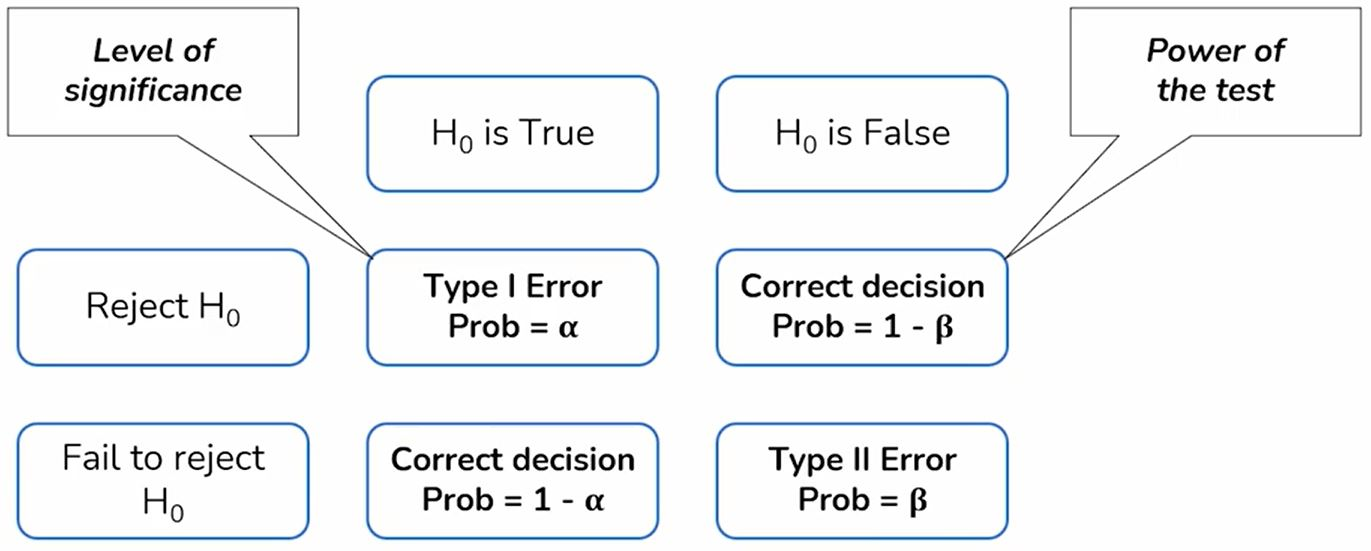
\includegraphics[height=2.5in]{type1andtype2errors}
		\caption{Hypothesis testing errors.}
		\label{fig:type1andtype2errors}
	\end{figure}

	\begin{numberedlist}
		\item Identify the key questions.
		\item Establish the hypotheses.
		\item Understand and prepare data.
		\item Identify the right test.
		\item Check the assumptions.
		\item Perform the test.
	\end{numberedlist}